
%(BEGIN_QUESTION)
% Copyright 2007, Tony R. Kuphaldt, released under the Creative Commons Attribution License (v 1.0)
% This means you may do almost anything with this work of mine, so long as you give me proper credit

A technician is troubleshooting a problem with a PLC program she just wrote.  The program is a simple motor start/stop control, with an HMI panel interfacing with the Siemens S7-200 PLC for another set of start/stop ``buttons'' to complement the hard-wired momentary-contact pushbuttons:

$$\includegraphics[width=15.5cm]{i03595x01.eps}$$

The problem is, the motor starts and stops just fine by pushing the real pushbuttons, but not by pressing the ``button'' objects on the HMI's touch-screen display.  For some reason, the HMI is unable to either start or stop the motor.  The tagname database programmed into the HMI only has two tags: {\tt Motor\_Start} and {\tt Motor\_Stop}, assigned (with ``write'' permission) to addresses {\tt I0.0} and {\tt I0.1} respectively.

\vskip 10pt

Identify what the problem is in this newly-programmed system, and also how to fix it.  Additionally, determine whether the pushbutton switch inputs are wired to {\it source} current to the PLC or {\it sink} current from it.

\vskip 20pt \vbox{\hrule \hbox{\strut \vrule{} {\bf Suggestions for Socratic discussion} \vrule} \hrule}

\begin{itemize}
\item{} If the ``Start'' pushbutton switch's wire came disconnected from input {\tt I0.0}, would the HMI panel then be able to start up the motor?
\item{} If the ``Stop'' pushbutton switch's wire came disconnected from input {\tt I0.1}, would the HMI panel then be able to stop the motor?
\item{} If the ``Start'' and ``Stop'' pushbutton switches were re-wired to connect to inputs {\tt I0.5} and {\tt I0.6} respectively, would this solve the problem?
\end{itemize}

\underbar{file i03595}
%(END_QUESTION)





%(BEGIN_ANSWER)

Both pushbutton switches are {\it sourcing} current to the PLC's inputs.

\vskip 10pt

I'll let you figure out what the problem is in this system.  {\it Hint: it's a very common mistake made by students first learning how to interface HMIs with PLCs}.

%(END_ANSWER)





%(BEGIN_NOTES)

There is a conflict between the real-world switch inputs writing to addresses {\tt I0.0} and {\tt I0.1}, versus the HMI panel trying to write data to those same addresses.  If the real-world inputs are scanned by the PLC immediately prior to execution of the PLC's program, then any data from the HMI panel will be over-written and thus ignored.





\vskip 20pt \vbox{\hrule \hbox{\strut \vrule{} {\bf Virtual Troubleshooting} \vrule} \hrule}

This question is a good candidate for a ``Virtual Troubleshooting'' exercise.  Presenting the diagram to students, you first imagine in your own mind a particular fault in the system.  Then, you present one or more symptoms of that fault (something noticeable by an operator or other user of the system).  Students then propose various diagnostic tests to perform on this system to identify the nature and location of the fault, as though they were technicians trying to troubleshoot the problem.  Your job is to tell them what the result(s) would be for each of the proposed diagnostic tests, documenting those results where all the students can see.

During and after the exercise, it is good to ask students follow-up questions such as:

\begin{itemize}
\item{} What does the result of the last diagnostic test tell you about the fault?
\item{} Suppose the results of the last diagnostic test were different.  What then would that result tell you about the fault?
\item{} Is the last diagnostic test the best one we could do?
\item{} What would be the ideal order of tests, to diagnose the problem in as few steps as possible?
\end{itemize}

%INDEX% PLC, troubleshooting: HMI address write conflict

%(END_NOTES)


